%!TEX root = ../main.tex
% file: problem1.tex
\section{Continued Fraction Representation Using an Iterator} % (fold)
\label{sec:continued_fraction_representation_using_an_iterator}
The first problem outlines the need to program a script with the ability to give the continued fraction representation of any number. We seek to do so by creating a class which contains our subroutines, one of which is an iterator allowing the user to take individual steps when seeking the result.

We begin by defining a continued fraction taking the form,
\begin{equation}
    L = a_0 + + \cfrac{1}{a_1
              + \cfrac{1}{a_2
              + \cfrac{1}{\ddots
              + \cfrac{1}{a_n}}}}
\end{equation}
The solution may be found by performing a series of integer divisions.
\subsection{Program Description} % (fold)
\label{sub:program_description}
In order to find a list of continued fractions, we define a function which performs a single step, finding a single convergent.
\begin{lstlisting}[caption={Calculation of a single convergent}, label=lst:convCalc,firstnumber=8]
    def step(self):
        """takes a step in the continued fraction representation"""
        out = self.x // self.n # // is integer division in python 2.2+
        self.n, self.x = self.x-self.n*out, self.n
        self.output.append(int(out))
        return int(out)
\end{lstlisting}\noindent
In Listing \ref{lst:convCalc} we see that the function operates on two class variables, the numerator and denominator named \emph{self.x} and \emph{self.n} respectively. By default, the denominator is specified as 1 in the initialization of the method, allowing for the user to either input a fraction or float to the class. 
\begin{lstlisting}[caption={Class iterator}, label=lst:iterator,firstnumber=15]
    def next(self):
        """this is our iterator"""
        if self.n:
            return self.step()
        else:
            raise StopIteration("You have exceeded the number of terms")
\end{lstlisting}\noindent
For the second portion of the problem, we are required to use an iterator to allow the user to iterate as they choose. The method shown in Listing \ref{lst:iterator} shows the use of an iterator to return a single convergent which is usable in a list comprehension. Similarly, we see that the iterator checks whether more convergents may be calculated prior to performing a step; if the user attempts return a convergent which does not exist we raise an exception.
% subsection program_description (end)

\subsection{Results} % (fold)
\label{sub:results}
We detail a set of tests to perform on the script. The first is agreement with the assignment, calculation of the continued fraction of 2.25. Similarly to check the fractional output (in addition to what was assigned) we input a value of 9/4. The final test is comparison against the widely available continued fraction of $\pi$, which was pulled from the internet for comparison.

\begin{figure}[H]
    \centering
        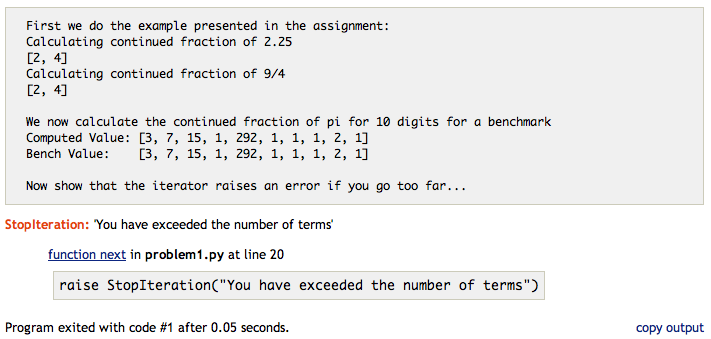
\includegraphics[height=3in, trim=0 .2in 0 0]{include/prob1test.png}
    \caption{Output generated from test routine for Problem 1}
    \label{fig:include_prob1test}
\end{figure}\noindent
The results of Figure \ref{fig:include_prob1test} show that the continued fraction of $2.25 (9/4)$ is indeed $[2,4]$ as we are shown in the handout. Similarly, the script produces the correct result for the first 10 convergents of $\pi$.
The final requirement was that the script produce an exception if the user attempts to perform more iterations than there are coefficients. This is shown in Fig. \ref{fig:include_prob1test} by the exception \emph{StopIteration}.
% subsection results (end)
% section continued_fraction_representation_using_an_iterator (end)